\documentclass[a4paper,oneside]{book}
\usepackage{caption}
\usepackage{subcaption}
\usepackage{enumitem}
\usepackage[english]{babel}
\usepackage{amsthm}
\usepackage{amssymb}
\newtheorem{theorem}{Theorem}[section]
\newtheorem{lemma}[theorem]{Lemma}
\renewcommand\qedsymbol{$\blacksquare$}
\usepackage[super]{nth}
\usepackage{geometry}
 \geometry{
 a4paper,
 total={170mm,257mm},
 left=20mm,
 top=20mm,
 }
\bibliographystyle{plain}
\usepackage{indentfirst}
\usepackage{csquotes}
\usepackage{graphicx}
\usepackage{wrapfig}
\graphicspath{ {./src/} }
\usepackage{hyperref}
\hypersetup{
    colorlinks=true,
    linkcolor=blue,
    filecolor=magenta,
    urlcolor=cyan,
}
\usepackage[linguistics]{forest}
\usepackage{ragged2e}
\usepackage{array}
\usepackage{booktabs}
\newcolumntype{R}[1]{>{\RaggedLeft\arraybackslash}p{#1}}
\newcolumntype{C}[1]{>{\Centering\arraybackslash}p{#1}}
\usepackage{amsmath}
\newcommand{\boxalign}[2][0.97\textwidth]{
 \par\noindent\tikzstyle{mybox} = [draw=black,inner sep=6pt]
 \begin{center}\begin{tikzpicture}
  \node [mybox] (box){%
   \begin{minipage}{#1}{\vspace{-5mm}#2}\end{minipage}
  };
 \end{tikzpicture}\end{center}
}
\usepackage[boxed, ruled, linesnumbered]{algorithm2e}
%% This declares a command \Comment
%% The argument will be surrounded by /* ... */
\SetKwComment{Comment}{/* }{ */}
\SetKw{Continue}{continue}
\usepackage{multicol}
\usepackage{listings}
\lstset{
basicstyle=\small\ttfamily,
breaklines=true
}
\usepackage{longtable}

\begin{document}

\clearpage
%% temporary titles
% command to provide stretchy vertical space in proportion
\newcommand\nbvspace[1][3]{\vspace*{\stretch{#1}}}
% allow some slack to avoid under/overfull boxes
\newcommand\nbstretchyspace{\spaceskip0.5em plus 0.25em minus 0.25em}
% To improve spacing on titlepages
\newcommand{\nbtitlestretch}{\spaceskip0.6em}
\pagestyle{empty}
\begin{center}
    \bfseries
    \nbvspace[1]
    \Huge
    {\nbtitlestretch\huge
        The \nth{2}-shortest Path}

    \nbvspace[1]
    \normalsize

    Project 3 Report\\
    Fundamental of Data Structure (2023 Fall)\\
    Zhejiang University
    \nbvspace[1]
    \small BY\\
    \Large Author Name\\[0.5em]
    \footnotesize Student ID: \\
    Teacher: HongHua Gan

    \nbvspace[2]
    Accomplished on December 2, 2023
    \nbvspace[3]
    \normalsize

    Made\\
    \large
    With \LaTeX
    \nbvspace[1]
\end{center}

\chapter*{Declaration}

I hereby declare that all the work done in this project titled ``The \nth{2}-shortest Path'' is of my independent effort.

\tableofcontents

\chapter{Introduction}

\section{Problem Description}

Give a \textbf{directed} graph $G = (V, E)$, where $V$ is the set of vertices and $E$ is the set of edges. Each edge $e \in E$ has a non-negative weight $w(e)$. Given two vertices $s$ and $t$, find the \nth{2}-shortest path from $s$ to $t$.

The graph \textbf{can} contain \textbf{cycles, self-loops and parellel edges}. For example:

\begin{figure}[!ht]
    \centering
    \caption{Structures in the graph}
    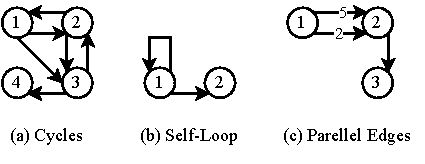
\includegraphics[width=0.5\textwidth]{src/graph_type.drawio.pdf}
\end{figure}

Note that the \textbf{end vertex} cannot have any outgoing edges. As TA said:

\begin{displayquote}
Although the question does not say it clearly, according to the meaning of the question, Lisa wants to go home, but it does not follow the shortest path but the shortest path, so once she reaches the end station $M$, it should be considered that she is going home.
\end{displayquote}

If there are multiple \nth{2}-shortest paths, we can output any of them. If there is no \nth{2}-shortest path, should inform the user.

\section{Problem Background}

This problem is a generalization of the shortest path problem. The shortest path problem is the problem of finding a path between two vertices (or nodes) in a graph such that the sum of the weights of its constituent edges is minimized. The best known algorithm for this problem is Dijkstra's algorithm, which runs in $O(|E| + |V| \log |V|)$ time. The algorithm was conceived by computer scientist Edsger W. Dijkstra in 1956 and published three years later.

We consider a long-studied generalization of the shortest path problem, in which not one but several short paths must be produced. The $k$ shortest paths problem is to list the $k$ paths connecting a given source-destination pair in the digraph with minimum total length. Our techniques also apply to the problem of listing all paths shorter than some given threshhold length. In the version of these problems studied here, cycles of repeated vertices are allowed. We first present a basic version of our algorithm, which is simple enough to be suitable for practical implementation while losing only a logarithmic factor in time complexity. We then show how to achieve optimal time (constant time per path once a shortest path tree has been computed) by applying Frederickson's algorithm for finding the minimum $k$ elements in a heap-ordered tree.

The \nth{2}-shortest path problem is a simpler version of the $k$ shortest path problem. Because you just care about the \nth{2}-shortest path, you don't need to maintain a list and find the $k$ shortest paths.

\chapter{Algorithm Specfication}
\label{chap:algorithm}

\section{Data Structure}

I use adjacency list to represent the graph. The graph is stored in a \verb|Graph| struct. The \verb|Graph| struct contains a \verb|Vertex| pointer array \verb|vertices| and a \verb|numVertices| field. The \verb|Vertex| struct contains two \verb|int| fields \verb|dest| and \verb|distance|, representing one outgoing edge and its weight. The \verb|Vertex| struct also contains a \verb|Vertex| pointer \verb|next|, representing the next vertex in the adjacency list.

\begin{figure}[!ht]
    \centering
    \caption{Data structure of the graph}
    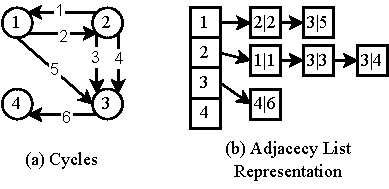
\includegraphics[width=0.5\textwidth]{src/ds.drawio.pdf}
\end{figure}

\section{Algorithm}

I use breadth-first search (BFS) to find the shortest path from $s$ to $t$. The algorithm is shown below:

\begin{algorithm}[H]
    \caption{BFS Algorithm}\label{alg:1}
    \DontPrintSemicolon
    \KwIn{Path $P$ from $s$ to $q_i$}
    \KwOut{Pathes $P'_k$ from $s$ to $q_{i+1}$ that are derived from $P$}
    \BlankLine
    \If{$q_i$ has no outgoing edges}{
        \Return{NULL}\;
    }
    $P' \gets P$\;
    \ForAll{$e \in E(q_i)$}{
        $P' \gets P' + e$\;
    }
    \Return{$P'_k$}\;
\end{algorithm}

All the pathes that haven't reached $t$ are stored in a priority queue, so BFS will always pop the current shortest path from the queue and explore it. If the path reaches $t$, we need to determine whether it is the \nth{2}-shortest path. If it is, we output it. If it is not, we continue to explore the next shortest path.

\begin{algorithm}[H]
    \caption{2-nd Selection Algorithm}\label{alg:2}
    \DontPrintSemicolon
    \KwIn{Graph $G$, start vertex $s$, end vertex $t$}
    \KwOut{The 2th-shortest path from $s$ to $t$}
    \BlankLine
    $Q \gets \emptyset$\;
    $Q.push(s)$\;
    \While{$Q$ is not empty}{
        $P \gets Q.pop()$\;
        \If{$P$ reaches $t$}{
            \eIf{$P$ is the 2th-shortest path}{
                \Return{$P$}\;
            }{
                \Continue\;
            }
        }
        \ForAll{$P' \in BFS(P)$}{
            $Q.push(P')$\;
        }
    }
    \Return{NULL}\;
\end{algorithm}

To determine whether a path is the \nth{2}-shortest path is simple. We just need to compare the length of the path with the length of the shortest path. When we first encountered $t$, the path is the shortest path. Record this length. When we encountered $t$ again, the path is the \nth{2}-shortest path if and only if the length of the path is not equal to the length of the shortest path.

It is worth noting that without the existence of a sub-shortest path, breadth-first search may get stuck in a loop, causing the algorithm's loop condition \verb|Q.isNotEmpty()| to never terminate, as shown in the diagram below. Therefore, when stepping through each path, it should be checked whether it has become trapped in a loop. Below, I will provide a proof that if a path passes through the same node more than twice, then it is definitely not a \nth{2} path. For such paths, they can be directly discarded.

\begin{figure}[!ht]
    \centering
    \caption{Bad Loop}
    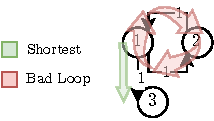
\includegraphics[width=0.25\textwidth]{src/bad_loop.drawio.pdf}
\end{figure}

\begin{theorem}\label{thm:1}
    Let $P$ be a path containing vertices $v_1, v_2, \dots, v_n$. If $P$ passes through $v_i$ more than twice, then $P$ is not a \nth{2} path.
\end{theorem}

\begin{proof}
    Starting from the first appearance of $v_i$, we can divide $P$ into parts $P_1, P_2, \dots, P_k$, where $P_1$ is the path from the start vertex to the first appearance of $v_i$, $P_k$ is the path from the last appearance of $v_i$ to the end vertex, and $P_j$ is the path from the $(j-1)$th appearance of $v_i$ to the $j$th appearance of $v_i$. Obviously, $P_1, P_2, \dots, P_k$ are all loops that pass through $v_i$. Each loop $P_j$ have a length of at least 0, and there must be a smallest loop $P_s$. If a path passes through $v_i$, then the \nth{2} shortest path must passes through $P_s$ and then never passes through $v_i$ again (otherwise it will form a longer loop). Therefore, if a path passes through $v_i$ more than twice, then it is definitely not a \nth{2} path.
\end{proof}

Actually, by induction, we can prove that if a path passes through the same node more than $k$ times, then it is definitely not a $k$th path. The proof is left to the reader.

\section{Program Architecture}

The picture below shows the architecture of the program. The input will be parsed into a graph. Then the program will run the \nth{2}-shortest path algorithm relying the \verb|PathPQ| priority queue. Finally, the program will output the result.

\begin{figure}[!ht]
    \centering
    \caption{Sketch of the program}
    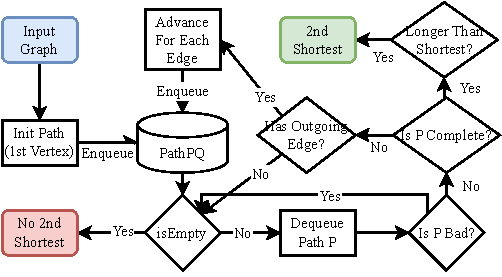
\includegraphics[width=0.8\textwidth]{src/program.drawio.pdf}
\end{figure}

\chapter{Test Cases}

\section{Table of Test Cases}

I've prepared a complete test suite for the program in \verb|code/testdata|. Some of the test cases are shown in Table \ref{tab:test_cases}.

\begin{longtable}{|c|p{3cm}|p{3.6cm}|p{3.6cm}|c|}
    \caption{Test Results}\label{tab:test_results} \\
\hline
\multicolumn{5}{| c |}{Begin of Table}\\
\hline
    No.                                                              & Purpose                                               & Input                                                             & Output                                                                          & Correctness \\ \hline
\endfirsthead

\hline
\multicolumn{5}{|c|}{Continuation of Table \ref{tab:test_results}}\\
\hline
    No.                                                              & Purpose                                               & Input                                                             & Output                                                                          & Correctness \\ \hline
\endhead

\hline
\endfoot

\hline
\multicolumn{5}{| c |}{End of Table}\\
\hline\hline
\endlastfoot

    1   & \verb|pta.in|\newline{} PTA provided test 
        &\lstinline!5 6!\newline{}\lstinline!1 2 50!\newline{}\lstinline!...!
        &\lstinline!240 1 2 4 5!
        &Yes\\ \hline
    2   & \verb|2.in|\newline{} Simple test 2
        &\lstinline!6 9!\newline{}\lstinline!1 2 10!\newline{}\lstinline!...!
        &\lstinline!7 1 5 3 4 2 6!
        &Yes\\ \hline
    3   & \verb|3.in|\newline{} Simple test 3
        &\lstinline!9 20!\newline{}\lstinline!1 4 546!\newline{}\lstinline!...!
        &\lstinline!1015 1 4 7 9!
        &Yes\\ \hline
    4   & \verb|loop1.in|\newline{} Single loop test
        & \lstinline!5 5!\newline{}\lstinline!1 2 1!\newline{}\lstinline!...!
        & \lstinline!10 1 2 3 4 2 3 5!
        & Yes\\ \hline
    5   & \verb|loop2.in|\newline{} (comprehensive) \newline{}Multiple loop test
        & \lstinline!6 7!\newline{}\lstinline!1 2 1!\newline{}\lstinline!...!
        & \lstinline!13 1 2 3 5 2 3 6!
        & Yes\\ \hline
    6   & \verb|extreme.in|\newline{} (largest) \newline{}Extreme test
        & \lstinline!1000 5000!\newline{}\lstinline!1 2 2!\newline{}\lstinline!...!\newline{}\lstinline!977 989 6!
        & \lstinline!63 1 95 216 556 1000!
        & Yes\\ \hline
    7   & \verb|no_2nd.in|\newline{} No \nth{2}-shortest path test
        & \lstinline!3 2!\newline{}\lstinline!1 2 1!\newline{}\lstinline!2 3 2!
        & \lstinline![Error] No second shortest path.!
        & Yes\\ \hline
    8   & \verb|one.in|\newline{} (smallest) \newline{} One node test
        & \lstinline!1 0!
        & \lstinline![Error] No second shortest path.!
        & Yes\\ \hline
    9  & \verb|self.in|\newline{} (extreme) \newline{} Self-loop test
        & \lstinline!3 5!\newline{}\lstinline!1 1 1!\newline{}\lstinline!...!
        & \lstinline!3 1 1 2 3!
        & Yes\\ \hline
    10  & \verb|para.in|\newline{} (extreme) \newline{} Parallel edge test
        & \lstinline!2 2!\newline{}\lstinline!1 2 1!\newline{}\lstinline!1 2 2!
        & \lstinline!2 1 2!
        & Yes\\ \hline
    11  & \verb|mid.in|\newline{} Middle vertex test
        & \lstinline!100 200!\newline{}\lstinline!1 2 9!\newline{}\lstinline!...!
        & \lstinline!68 1 7 8 36 70 100!
        & Yes\\ \hline
\end{longtable}

\section{Visualization}

Their visualized graphs are shown in Figure \ref{fig:test_graphs}.

\begin{figure}[!ht]
    \centering
    \caption{Test Graphs}
    \begin{subfigure}[b]{0.3\textwidth}
        \centering
        \caption{pta.in}
        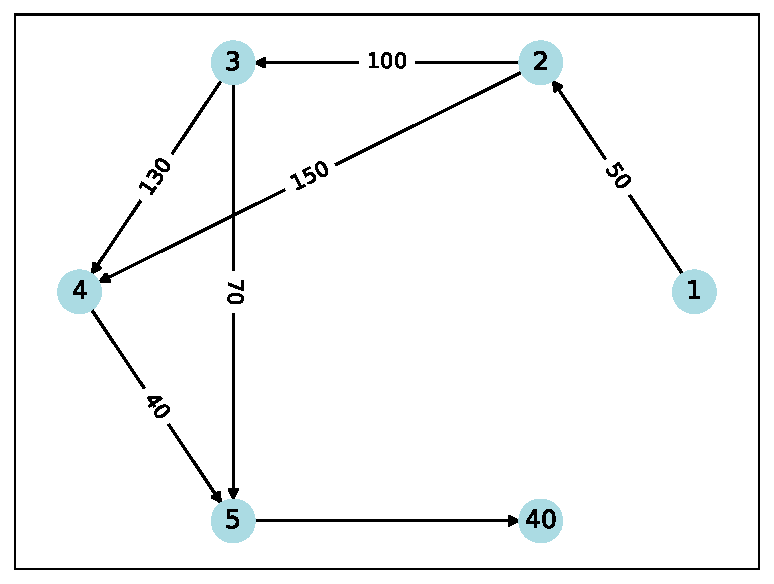
\includegraphics[width=\textwidth]{src/pta.pdf}
    \end{subfigure}
    \begin{subfigure}[b]{0.3\textwidth}
        \centering
        \caption{2.in}
        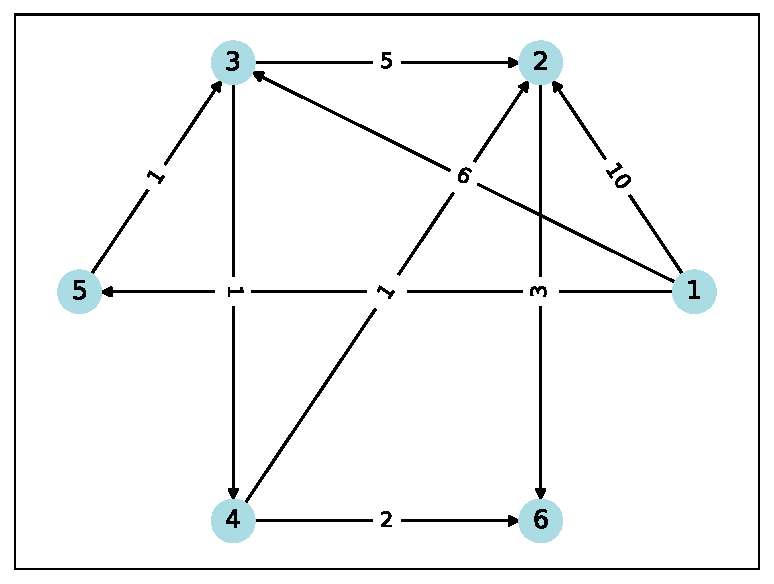
\includegraphics[width=\textwidth]{src/2.pdf}
    \end{subfigure}
    \begin{subfigure}[b]{0.3\textwidth}
        \centering
        \caption{3.in}
        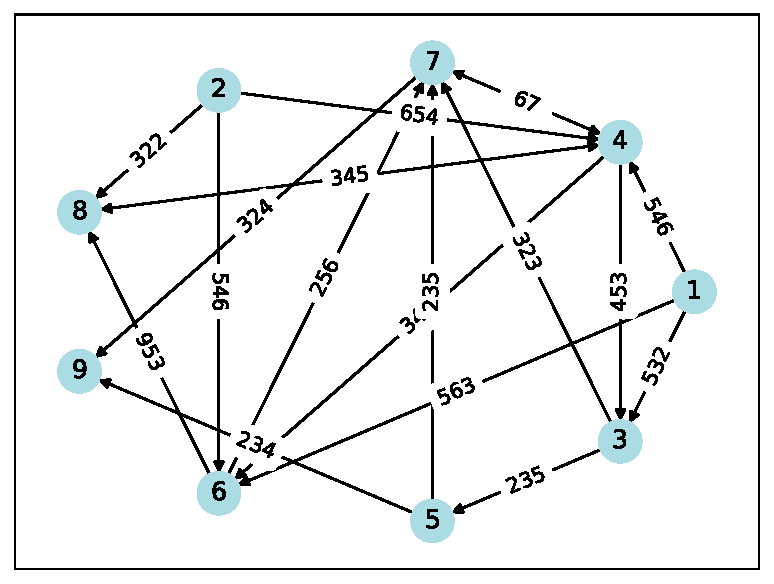
\includegraphics[width=\textwidth]{src/3.pdf}
    \end{subfigure}
    \begin{subfigure}[b]{0.3\textwidth}
        \centering
        \caption{loop1.in}
        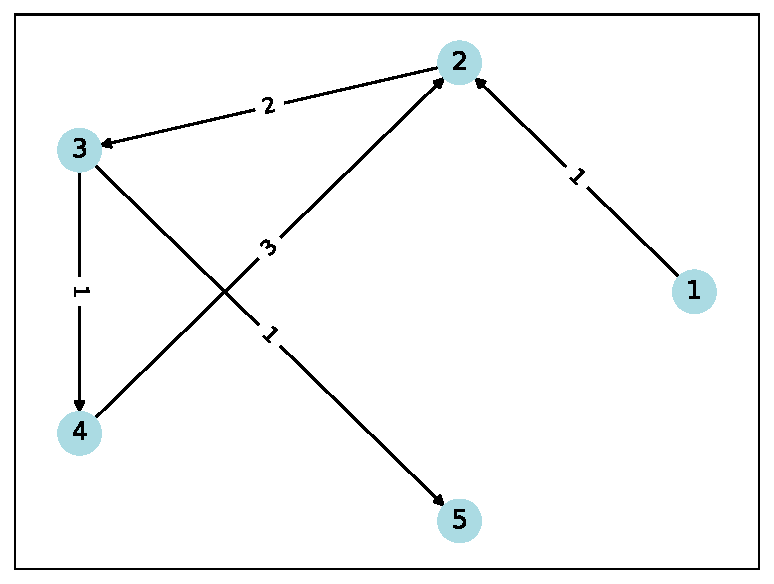
\includegraphics[width=\textwidth]{src/loop1.pdf}
    \end{subfigure}
    \begin{subfigure}[b]{0.3\textwidth}
        \centering
        \caption{loop2.in}
        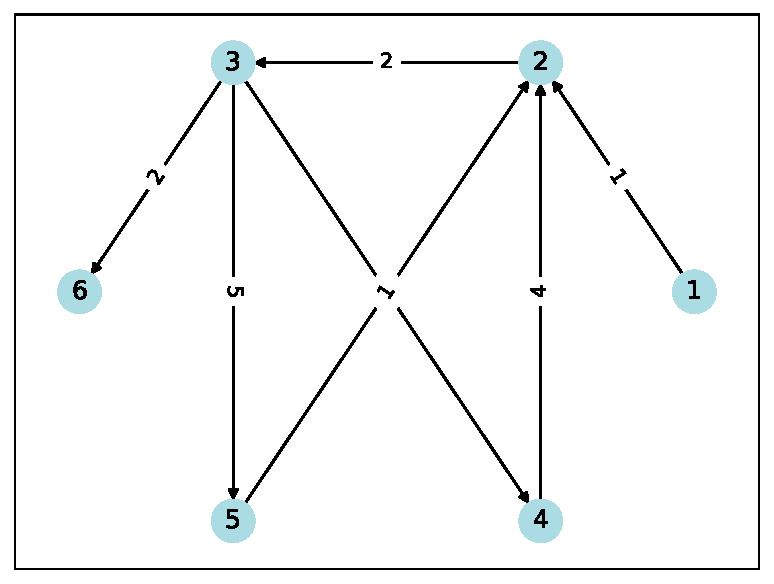
\includegraphics[width=\textwidth]{src/loop2.pdf}
    \end{subfigure}
    \begin{subfigure}[b]{0.3\textwidth}
        \centering
        \caption{extreme.in}
        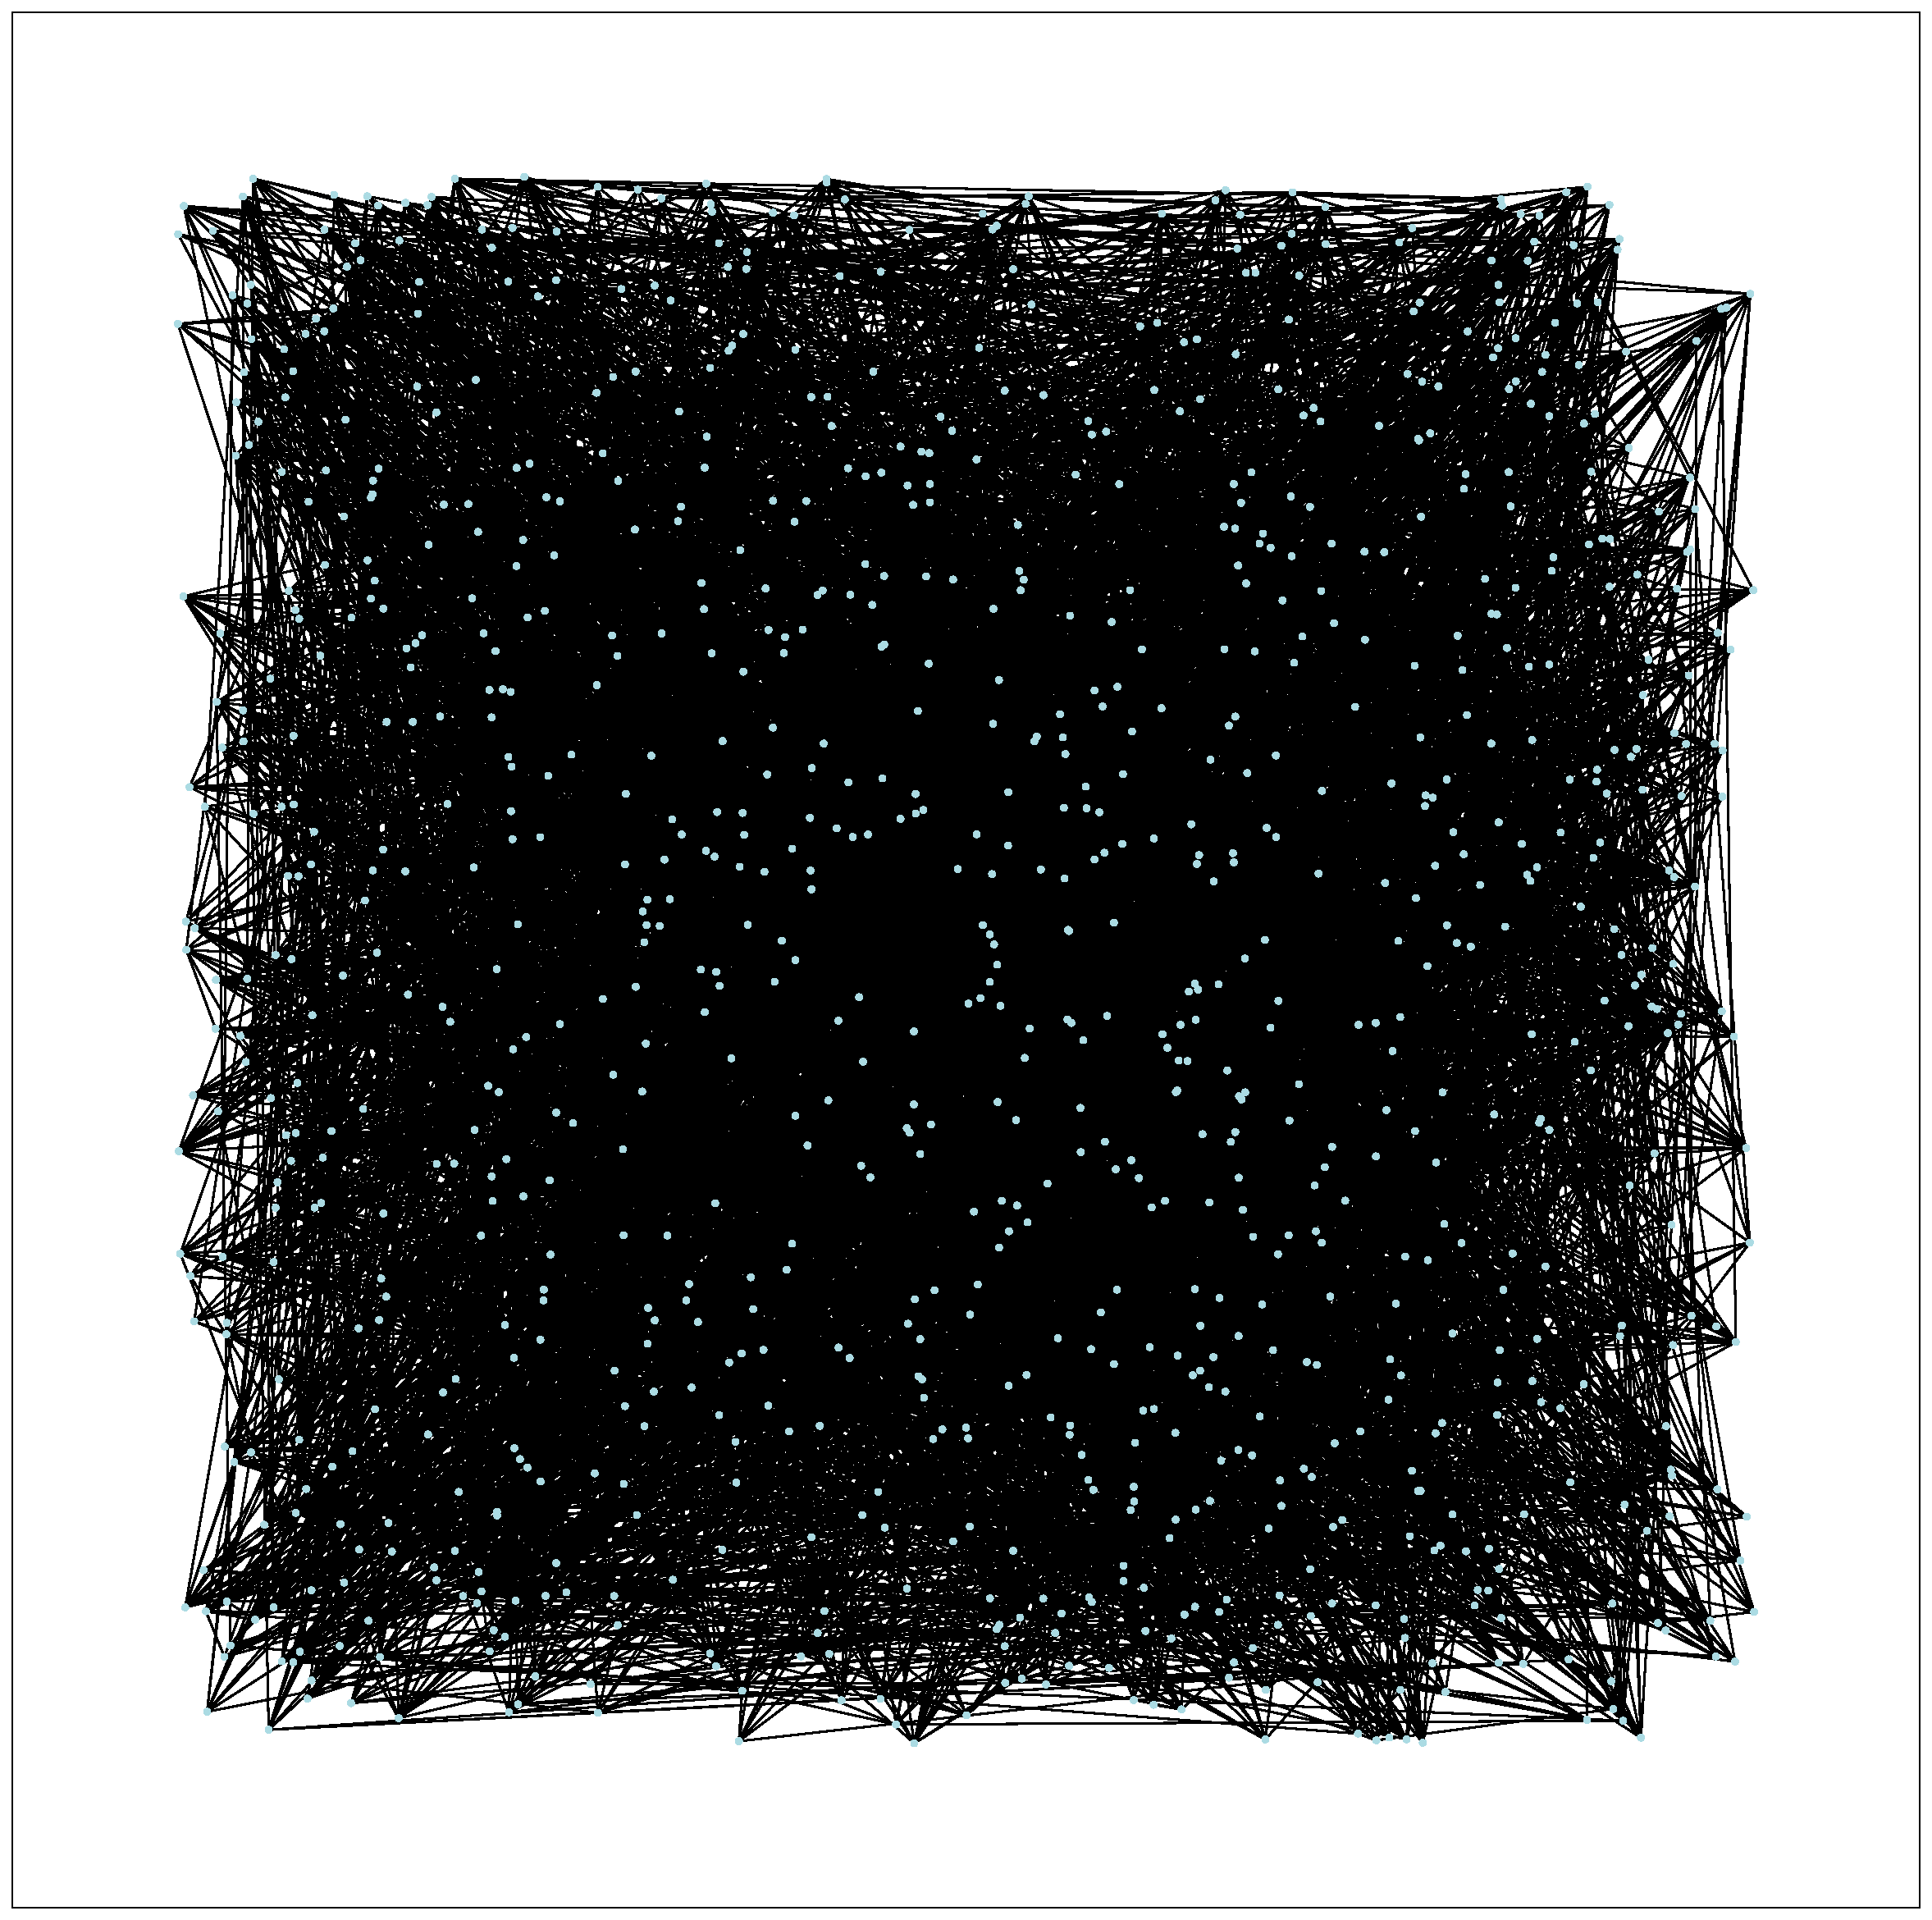
\includegraphics[width=\textwidth]{src/extreme.pdf}
    \end{subfigure}
    \begin{subfigure}[b]{0.3\textwidth}
        \centering
        \caption{no\_2nd.in}
        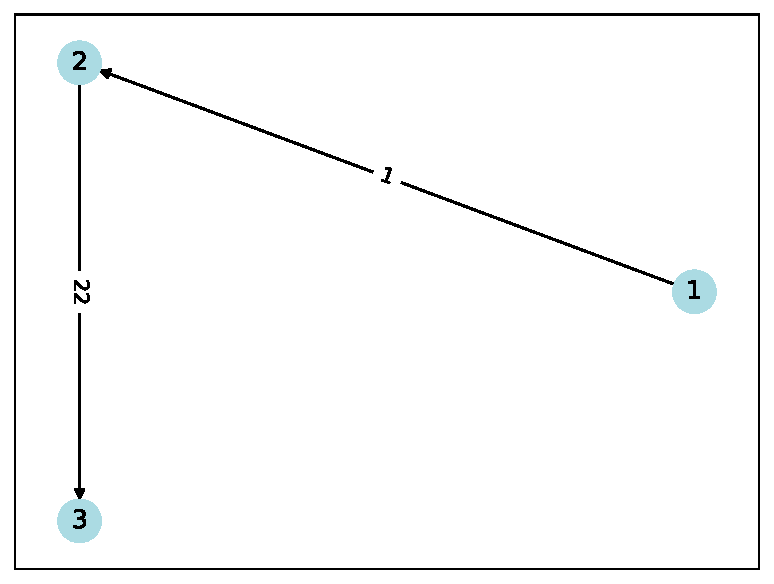
\includegraphics[width=\textwidth]{src/no_2nd.pdf}
    \end{subfigure}
    \begin{subfigure}[b]{0.3\textwidth}
        \centering
        \caption{one.in}
        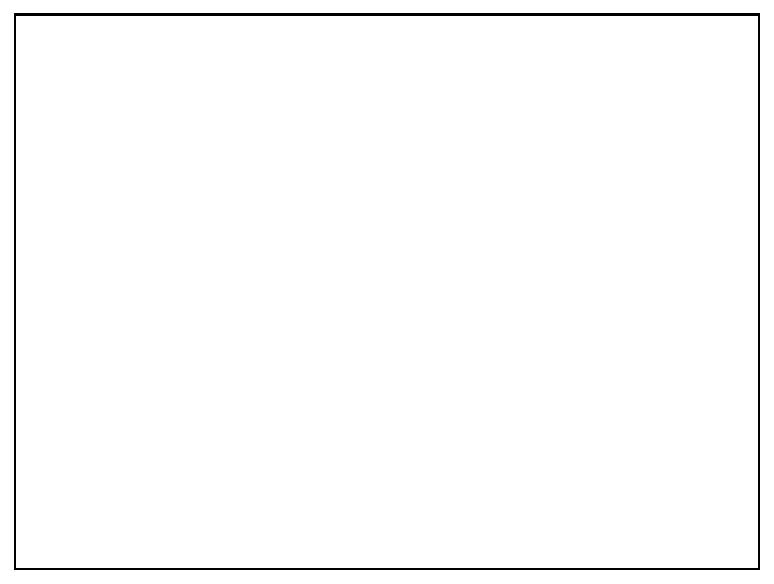
\includegraphics[width=\textwidth]{src/one.pdf}
    \end{subfigure}
    \begin{subfigure}[b]{0.3\textwidth}
        \centering
        \caption{self.in}
        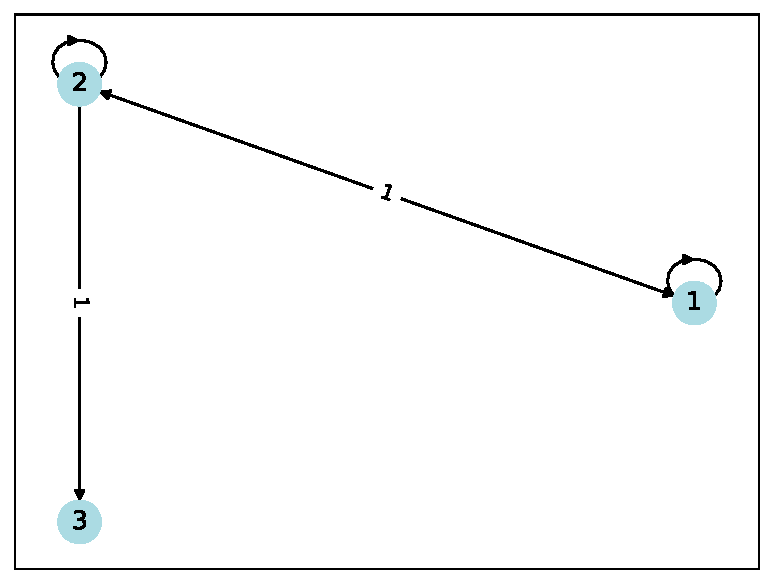
\includegraphics[width=\textwidth]{src/self.pdf}
    \end{subfigure}
    \begin{subfigure}[b]{0.3\textwidth}
        \centering
        \caption{para.in}
        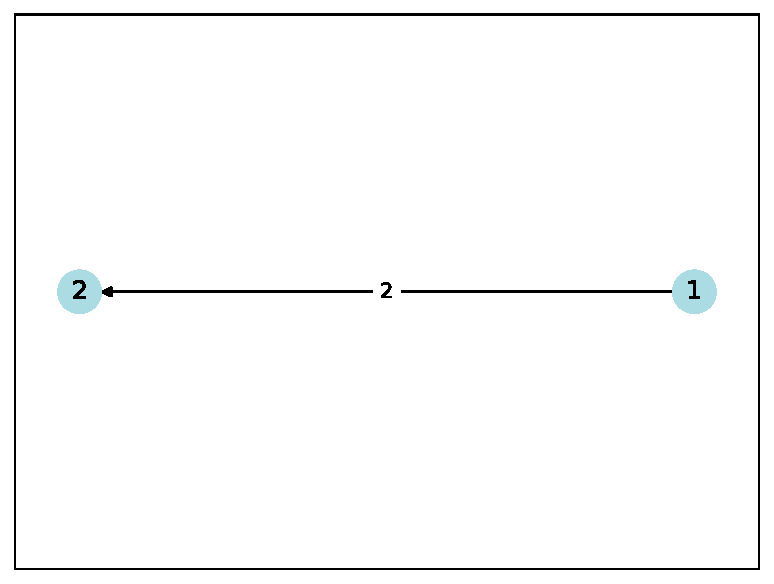
\includegraphics[width=\textwidth]{src/para.pdf}
    \end{subfigure}
    \begin{subfigure}[b]{0.3\textwidth}
        \centering
        \caption{mid.in}
        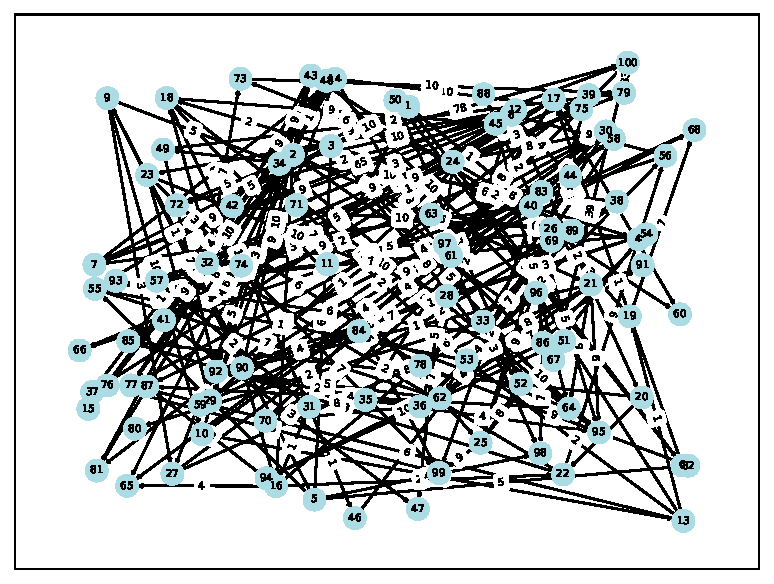
\includegraphics[width=\textwidth]{src/mid.pdf}
    \end{subfigure}
    \label{fig:test_graphs}
\end{figure}

\chapter{Analysis and Comments}

\section{Time Complexity}

\begin{theorem}
The time complexity of the algorithm is $O(|E| + |V| \log |V|)$.
\end{theorem}

\begin{proof}
    Analyse the time complexity of the algorithm step by step.

    \begin{itemize}[leftmargin=4em]
        \item[Step I] Construct the graph. The time complexity is $O(|E|)$.
        \item[Step II] Run BFS until the shortest path is found. This path must be a loopless path. The time complexity is $O(|V|)$.
        \item[Step III] The algorithm will run in two cases.
        \begin{itemize}[leftmargin=4em]
            \item[Case 1] Run BFS until the \nth{2}-shortest path is found. As shown Theorem \ref{thm:1}, the \nth{2}-shortest path can contain at most one loop, so the time complexity is $O(|V|)$. Before this path is found, the algorithm will sort the pathes in the priority queue. The time complexity is $O(|V| \log |V|)$.
            \item[Case 2] If no \nth{2}-shortest path is found, the algorithm will traverse all the pathes (containing at most one loop) in the priority queue. The time complexity is $O(|E|)$.
        \end{itemize}
        \item[Step IV] Output the result. The time complexity is $O(|V|)$.
    \end{itemize}
    Therefore, the time complexity of the algorithm is $O(|E| + |V| \log |V|)$.
\end{proof}

\section{Space Complexity}

\begin{theorem}
The space complexity of the algorithm is $O(|E| + |V|)$.
\end{theorem}

\begin{proof}
    The space complexity of the algorithm is the sum of the space complexity of the graph and the priority queue.

    The space complexity of the graph is $O(|E| + |V|)$.

    The space complexity of the priority queue is complicated. The priority queue contains all the pathes that haven't reached $t$. Because pathes with more than one loop are discarded, each path contains at most $2|E|$ vertices. The number of pathes in the priority queue is at most $|V|$ (BFS). Therefore, the space complexity of the priority queue is $O(|E| + |V|)$.

    In total, the space complexity of the algorithm is $O(|E| + |V|)$.
\end{proof}

\section{Comments}

Many papers study algorithms for k shortest paths \cite{doi:10.1137/S0097539795290477}. Dreyfus and Yen \cite{6d707c5e-cd30-3994-a0f9-2e2fa3dfc631} cite several additional papers on the subject going back as far as 1957.

One must distinguish several common variations of the problem. In many of the papers cited above, the paths are restricted to be simple, i.e. no vertex can be repeated. This has advantages in some applications, but as our results show this restriction seems to make the problem significantly harder. Several papers \cite{doi:10.1137/S0097539795290477} consider the version of the k shortest paths problem in which repeated vertices are allowed, and it is this version that we also study. Of course, for the DAGs that arise in many of the applications described above including scheduling and dynamic programming, no path can have a repeated vertex and the two versions of the problem become equivalent. Note also that in the application described earlier of listing the most likely failure paths of a system modelled by a finite state machine, it is the version studied here rather than the more common simple path version that one wants to solve.

\appendix

\chapter{Source Code}

\section{Source Code Statistics}

The source code is in the \verb|code| directory. I've commented the source code
using Doxygen-style comments.

\begin{enumerate}
    \item \verb|main.c|: Driver program.
    \item \verb|graph.c, graph.h|: Implementation of the expression tree.
\end{enumerate}

And here is the statistics of the source code above using \verb|cloc| tool:

\begin{verbatim}
-------------------------------------------------------------------------------
Language                     files          blank        comment           code
-------------------------------------------------------------------------------
C                                2             38            201            289
C/C++ Header                     1              8             21             45
-------------------------------------------------------------------------------
SUM:                             3             46            222            334
-------------------------------------------------------------------------------
\end{verbatim}

$39\%$ of the source code is well documented with Doxygen-style comments. This
satisfies the requirement of the project.

\section{Compilation and Execution}

The program is written in C and can be compiled using \verb|gcc|. There is a \verb|Makefile| in the \verb|code| directory. If you use UNIX system, you can compile the program by running \verb|make| in the \verb|code| directory.

If you use Windows system, you can compile the program by running the following command in the \verb|code| directory:

\begin{verbatim}
gcc -o main.exe main.c graph.c
\end{verbatim}

If you use IDE, you can also import the source code into the IDE and compile it.

After compilation, you can run the program by running \verb|main| or \verb|main.exe| in the \verb|code| directory.

The program will recognize the input from command line. If you want to input the expression from a file, you can run the program like this:

\begin{verbatim}
./main input.txt 
\end{verbatim}

If you don't specify the input file, the program will read the expression from standard input. You can redirect the input from a file like this:

\begin{verbatim}
./main < input.txt
\end{verbatim}

Or you can type the graph in the terminal.

I've prepared a complete test suite for the program in \verb|code/testdata|. If you use UNIX system, you can run the program on the test data by running the following command in the \verb|code| directory:

\begin{verbatim}
make test
\end{verbatim}

It will run the program on all the test data and save the output in \verb|code/testdata| with \verb|.out| suffix.

If you don't use UNIX system, you can test the program manually:

\begin{verbatim}
./main testdata/pta.in 
\end{verbatim}

\bibliography{report}

\end{document}